\providecommand{\swtodo}[1]{\textbf{[TODO: #1]}}

\usetikzlibrary{arrows.meta, positioning, calc, shapes.geometric, fit, patterns}

\tikzset{
  swbase/.style={draw, align=center, font=\footnotesize, inner sep=3pt,
                 line width=0.5pt,
                 execute at begin node={\hyphenpenalty=10000\relax\exhyphenpenalty=10000\relax}},
  swproc/.style={swbase, rectangle, minimum height=7mm, text width=#1},
  swproc/.default=34mm,
  swterm/.style={swbase, rectangle, rounded corners=3.4mm,
                 minimum height=7mm, text width=#1},
  swterm/.default=30mm,
  swdec/.style={swbase, diamond, aspect=2.4, inner sep=0.5pt, text width=#1},
  swdec/.default=24mm,
  % predefined process (detailed in another figure): box with side bars
  swsub/.style={swproc=#1, inner xsep=4.5mm,
    path picture={
      \draw[line width=0.5pt]
        ([xshift=1.6mm]path picture bounding box.north west) --
        ([xshift=1.6mm]path picture bounding box.south west)
        ([xshift=-1.6mm]path picture bounding box.north east) --
        ([xshift=-1.6mm]path picture bounding box.south east);}},
  swsub/.default=30mm,
  swarr/.style={-{Latex[length=2mm]}, line width=0.5pt},
  swdbl/.style={{Latex[length=2mm]}-{Latex[length=2mm]}, line width=0.5pt},
  swlbl/.style={font=\scriptsize, inner sep=1.5pt},
  swhw/.style={swbase, rectangle, minimum height=8mm, text width=#1,
               fill=black!10},
  swhw/.default=26mm,
}


% =====================================================================
%  Chapter 3 -- System Modeling & Theoretical Design
%
%  The Randles model and the capacitive current rejection derivation
%  now live in Chapter 2 (sec:cell_model and sec:dpv_theory).
%  The label sec:dpv_rejection was moved with them, so references to it
%  in Chapters 5 and 6 now point to the DPV subsection in Chapter 2.
% =====================================================================

\chapter{System Modeling \& Theoretical Design}
\label{chap:modeling}

This chapter presents the potentiostat designed for this project, referred to as the OpenStat. The OpenStat combines an integrated analog front-end, a browser interface and a standalone onboard display in a single handheld instrument. Section~\ref{sec:architecture} describes its architecture and the role of each part. Section~\ref{sec:afe_stability} then analyses the stability of the two amplifier loops that drive and measure the cell, which sets the requirements for the hardware in Chapter~\ref{chap:hardware_design} and the firmware in Chapter~\ref{chap:software_design}.

%------------------------------------------------------------------
\section{System Architecture}
\label{sec:architecture}

The OpenStat is built around two key elements. An AD5941 analog front-end applies the potential to the three-electrode cell and measures the resulting current. An ESP32-S3 controls the AD5941 over SPI, times the DPV waveform, computes the differential current and stores the results. The AD5941 was selected over a discrete design because it integrates the control amplifier, RE buffer and TIA of Section~\ref{sec:3opamp_topology} on a single chip, together with a 12-bit DAC, a 16-bit ADC and eight programmable gain ranges, at sub-milliwatt power in a millimetre-scale package. Its main limitation, the capped compliance voltage, does not restrict this application. In addition to these key elements are the interfaces that make the instrument standalone, namely a TFT display and SD card, the user interface, and a web server that serves results over Wi-Fi. Figure~\ref{fig:architecture} shows how the firmware connects these parts, with a single main loop servicing the measurement, display and web server in turn.

\begin{figure}[H]
  \centering
  \caption{Software architecture.
    Arrows show the direction of calls or data.}
  \label{fig:architecture}
  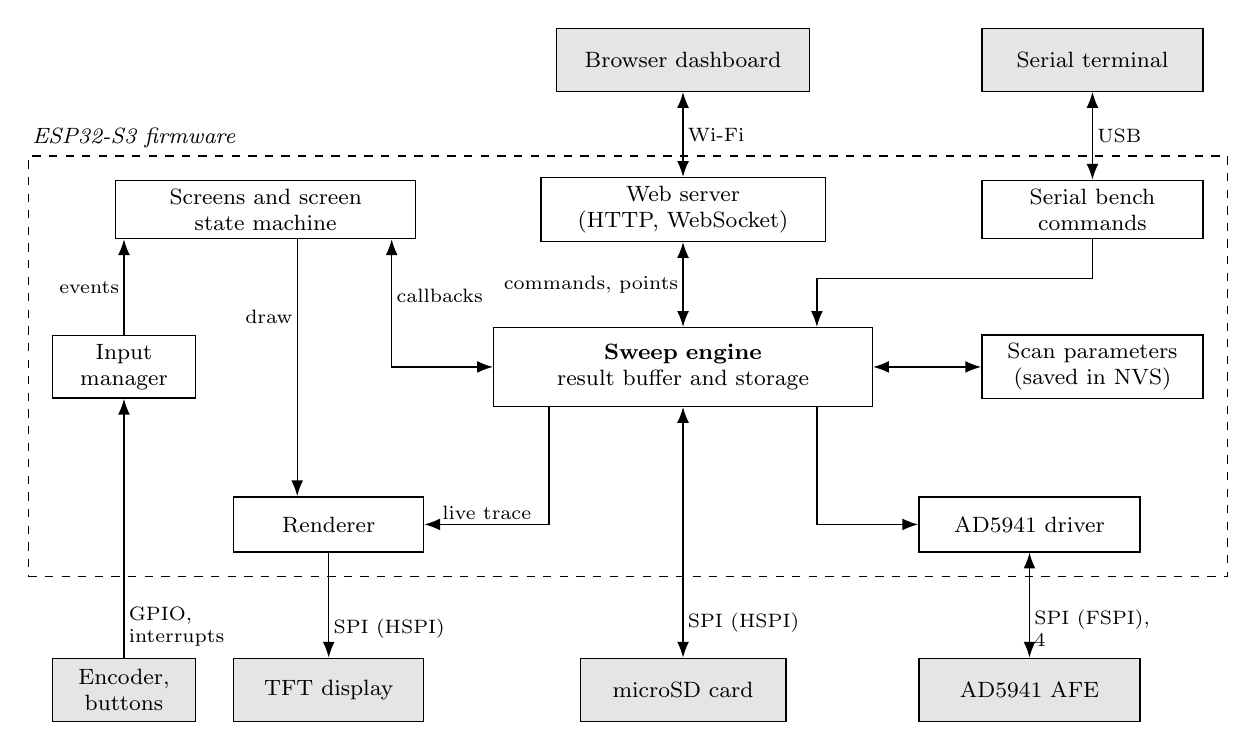
\begin{tikzpicture}[x=1cm, y=1cm]
    % --- external, top
    \node[swhw=30mm] (browser) at (7.6, 6.9) {Browser dashboard};
    \node[swhw=26mm] (pc)      at (12.8, 6.9) {Serial terminal};
    % --- row A
    \node[swproc=36mm] (screens) at (2.3, 5.0) {Screens and screen\\state machine};
    \node[swproc=34mm] (web)     at (7.6, 5.0) {Web server\\(HTTP, WebSocket)};
    \node[swproc=26mm] (serial)  at (12.8, 5.0) {Serial bench\\commands};
    % --- row B
    \node[swproc=16mm] (input)  at (0.5, 3.0) {Input\\manager};
    \node[swproc=46mm, minimum height=10mm] (engine) at (7.6, 3.0)
      {\textbf{Sweep engine}\\result buffer and storage};
    \node[swproc=26mm] (params) at (12.8, 3.0) {Scan parameters\\(saved in NVS)};
    % --- row C
    \node[swproc=22mm] (render) at (3.1, 1.0) {Renderer};
    \node[swproc=26mm] (driver) at (12.0, 1.0) {AD5941 driver};
    % --- firmware boundary
    \node[draw, dashed, line width=0.5pt, inner sep=3mm,
          fit=(screens)(serial)(input)(render)(driver)(params)] (fw) {};
    \node[swlbl, anchor=south west, font=\footnotesize\itshape]
      at ([yshift=0.3mm]fw.north west) {ESP32-S3 firmware};
    % --- hardware, bottom
    \node[swhw=16mm] (enc)  at (0.5, -1.1) {Encoder,\\buttons};
    \node[swhw=22mm] (tft)  at (3.1, -1.1) {TFT display};
    \node[swhw=24mm] (sd)   at (7.6, -1.1) {microSD card};
    \node[swhw=26mm] (afe)  at (12.0, -1.1) {AD5941 AFE};
    % --- connections
    \draw[swdbl] (browser) -- node[swlbl, right] {Wi-Fi} (web);
    \draw[swdbl] (pc) -- node[swlbl, right] {USB} (serial);
    \draw[swarr] (enc) -- node[swlbl, right, align=left, pos=0.12] {GPIO,\\interrupts} (input);
    \draw[swarr] (input.north) -- node[swlbl, left] {events}
      (input.north |- screens.south);
    \draw[swarr] ([xshift=-4mm]render.north |- screens.south) --
      node[swlbl, left, pos=0.3] {draw} ([xshift=-4mm]render.north);
    \draw[swdbl] ([xshift=16mm]screens.south) |-
      node[swlbl, right, pos=0.22] {callbacks} (engine.west);
    \draw[swarr] ([xshift=-17mm]engine.south) |-
      node[swlbl, above, pos=0.75] {live trace} (render.east);
    \draw[swdbl] (web) -- node[swlbl, left] {commands, points} (engine);
    \draw[swarr] (serial.south) -- ++(0,-0.5) -| ([xshift=17mm]engine.north);
    \draw[swdbl] (params) -- (engine);
    \draw[swarr] ([xshift=17mm]engine.south) |- (driver.west);
    \draw[swarr] (render) -- node[swlbl, right, pos=0.72] {SPI (HSPI)} (tft);
    \draw[swdbl] (engine) -- node[swlbl, right, pos=0.86] {SPI (HSPI)} (sd);
    \draw[swdbl] (driver) --
      node[swlbl, right, align=left, pos=0.72] {SPI (FSPI),\\\SI{4}{\mega\hertz}} (afe);
  \end{tikzpicture}
\end{figure}

The hardware that implements this architecture is described in Chapter~\ref{chap:hardware_design} and the firmware in Chapter~\ref{chap:software_design}. The rest of this chapter considers whether the analog front-end remains stable when the electrochemical cell is connected to it.

% ---------------------------------------------------------------------
\section{Analog Front-End Stability}
\label{sec:afe_stability}

The AD5941 implements the three-amplifier topology of Section~\ref{sec:3opamp_topology}. Its potentiostat amplifier acts as the control amplifier driving the CE, the RE is sensed through a high-impedance unity-gain stage, and the high-speed TIA holds the WE at virtual ground and converts the cell current to a voltage. The Randles model of Section~\ref{sec:cell_model} places specific demands on these amplifiers. The total resistance $R_s + R_{ct}$ sets the compliance voltage that the control amplifier must provide \cite{pineresearch_compliance}, and the time constant $R_sC_{dl}$ sets how long a DPV pulse must be held before the capacitive current has decayed \cite{bard2001}. The cell also lies inside the feedback loops of both the control amplifier and the TIA, so $C_{dl}$ affects the stability of each.

Each loop is assessed with the phase-margin criterion. The loop gain
$L(s) = A(s)\beta(s)$ is evaluated at the crossover frequency $\omega_c$,
where $|L(j\omega_c)| = 1$, and the phase margin
$\phi_\text{PM} = \SI{180}{\degree} + \angle L(j\omega_c)$ must be positive
for the loop to be stable, with \SIrange{45}{65}{\degree} giving a
well-damped response \cite{c2}. Both amplifiers are modeled with a single
dominant pole, $A(s) = \omega_t/s$ with $\omega_t = 2\pi \cdot
\text{GBW}$ \cite{bard2001}. The underlying feedback theory and the
derivations of the results below are given in Appendix~\ref{app:feedback}.

\subsection{Control Loop}
\label{sec:control_loop}

Only the high-frequency behaviour of the cell matters for stability. $R_{ct}$
and $Z_W$ in Figure~\ref{fig:randles_circuit} govern the slow Faradaic
response and are omitted, which reduces the cell to $C_{dl}$ in series with
the uncompensated resistance $R_u$, the part of $R_s$ between the RE and the
WE \cite{bard2001, c7, c8}. This reduced cell is shown in
Figure~\ref{fig:cell_buffer}.

\begin{figure}[H]
    \centering
    \caption{Electrochemical cell equivalent circuit interfaced with the reference electrode buffer.}
    \label{fig:cell_buffer}
    \begin{circuitikz}[american, thick]
        
        % Block style for the RE buffer
        \tikzset{
            re_block/.style={
                rectangle,
                draw=teal!50!black,
                fill=teal!80!black,
                text=white,
                rounded corners=3pt,
                minimum width=3.8cm,
                minimum height=1.2cm,
                align=center
            }
        }

        % 1. Left wire and CE node (Shifted left for clearance)
        \draw (2,0) -- (0.5,0);
        \fill (0.5,0) circle (2.5pt);
        \node[above=0.15cm] at (0.5,0) {\textbf{CE}};
        \node[below=0.15cm] at (-0.2,0) {\textsf{$e_o(s)$, Op-Amp A}};
        
        % Wire entering the dashed box
        \draw (0.5,0) -- (2.0,0);
        
        % 2. Resistor Ru
        \draw (2.0,0) to[R, l=$R_u$] (4.5,0);
        
        % 3. Center Tap (to RE buffer)
        \fill (4.5,0) circle (2.5pt);
        
        % 4. Capacitor Cdl
        \draw (4.5,0) to[C, l=$C_{dl}$] (7.0,0);
        
        % 5. Right wire, WE node, and Ground
        \draw (7.0,0) -- (8.5,0);
        \fill (8.5,0) circle (2.5pt);
        \draw (8.5,0) node[ground]{}; 
        
        % Adjusted WE label position to not clash with ground symbol
        \node[below=0.85cm, align=center] at (8.5,0) {\textbf{WE}\\ \textsf{Virtual ground (Op-Amp C, TIA)}};
        
        % 6. Dashed Box for Electrochemical Cell
        % Adjusted dimensions to encompass R and C properly and leave room for text
        \draw[dashed, draw=gray!80, thick] (1.6, -1.3) rectangle (7.4, 1.6);
        
        % Text shifted slightly inside the box so it doesn't overlap the border
        \node[anchor=north west, text=gray!90] at (1.7, -0.5) {\textsf{Electrochemical cell ($R_u$, $C_{dl}$)}};
        
        % 7. RE Buffer Block
        \node[re_block] (re_buffer) at (4.5, 2.7) {\textbf{RE buffer}\\ \textsf{Op-Amp B ($\beta\approx1$)}};
        
        % 8. Arrows to/from RE Buffer
        \draw[-stealth, thick] (4.5,0) -- (re_buffer.south);
        \draw[-stealth, thick] (re_buffer.north) -- (4.5, 4.4) node[above] {\textsf{\textbf{$E_{ref}(s)$ to summing junction}}};
        
    \end{circuitikz}
\end{figure}


The RE senses the voltage across $C_{dl}$, so the feedback factor is the
divider formed by $R_u$ and $C_{dl}$ (Appendix~\ref{app:beta}):
\begin{equation}
  \beta(s) = \frac{1}{1 + s\tau_\text{cell}},
  \qquad \tau_\text{cell} \equiv R_uC_{dl}.
  \label{eq:beta}
\end{equation}
The loop gain of the control amplifier is then
\begin{equation}
  L_\text{ctrl}(s) = \frac{\omega_{t,\text{ctrl}}}{s\,(1 + s\tau_\text{cell})},
  \label{eq:l_ctrl}
\end{equation}
which for $\omega \gg 1/\tau_\text{cell}$ crosses unity at
\begin{equation}
  \omega_{c,\text{ctrl}} \approx \sqrt{\frac{\omega_{t,\text{ctrl}}}{\tau_\text{cell}}}.
  \label{eq:wc_ctrl}
\end{equation}
At this frequency the integrator contributes \SI{-90}{\degree} and the cell
pole adds lag approaching a further \SI{-90}{\degree} as
$\omega_{c,\text{ctrl}}\tau_\text{cell}$ grows, so the phase margin falls as
$\tau_\text{cell}$ increases. $R_u$ is typically tens to a few hundred ohms
in a well-conducting aqueous electrolyte \cite{bard2001}, so
$\tau_\text{cell}$ is much smaller than the $R_fC_{dl}$ time constant of the
TIA loop (Section~\ref{sec:tia_loop}), and the control loop is the less
critical of the two. Because the gain-bandwidth product of the control
amplifier is fixed inside the AD5941, this loop cannot be compensated in the
design; instead it limits the cells that can be driven, since a
high-resistance sample or a large electrode raises $\tau_\text{cell}$ and
erodes the margin. The RE buffer is a voltage follower with $\beta = 1$;
because its open-loop gain is large across the frequencies of interest, it
contributes no significant pole \cite{c3}.

\subsection{TIA Loop and Compensation}
\label{sec:tia_loop}

The WE connects directly to the inverting input of the TIA, so $C_{dl}$ shunts this node in the same way that
the junction capacitance of a photodiode shunts the input of a photodiode
amplifier \cite{graeme1996photodiode}.

With a feedback resistor $R_f$, $C_{dl}$ introduces a zero into the noise
gain (Appendix~\ref{app:tia}),
\begin{equation}
  NG(s) = 1 + sR_fC_{dl},
  \qquad f_z = \frac{1}{2\pi R_fC_{dl}},
  \label{eq:noise_gain}
\end{equation}
which appears as a second pole in the loop gain:
\begin{equation}
  L_\text{TIA}(s) = \frac{A(s)}{NG(s)}
    = \frac{\omega_t}{s\,(1 + sR_fC_{dl})}.
  \label{eq:l_tia}
\end{equation}
For $\omega \gg 1/R_fC_{dl}$ the crossover frequency is
\begin{equation}
  \omega_{c,\text{TIA}} \approx \sqrt{\frac{\omega_t}{R_fC_{dl}}}.
  \label{eq:wc_tia}
\end{equation}
At this frequency both poles contribute close to \SI{-90}{\degree}, so the
phase margin collapses towards \SI{0}{\degree} and the TIA rings or
oscillates \cite{franco2014design}. Because $R_f$ must be large to resolve
nanoampere currents, $R_fC_{dl} \gg R_uC_{dl}$, which makes this the
critical loop.

The loop is stabilised by placing a capacitor $C_f$ in parallel with $R_f$.
$C_f$ adds a pole to the noise gain at $1/(2\pi R_fC_f)$, above the zero
caused by $C_{dl}$, which levels off the noise gain before it meets the
open-loop gain of the amplifier. Placing this pole at $f_z$ and the GBW gives a phase margin of about \SI{45}{\degree} or more
\cite{graeme1996photodiode, adi_mt059}, for which
\begin{equation}
  C_f = \sqrt{\frac{C_{dl}}{2\pi R_f \cdot \text{GBW}}}.
  \label{eq:cf}
\end{equation}
$C_f$ must therefore be sized for the largest expected $C_{dl}$ of the cell rather than chosen independently of it. In the AD5941, the capacitor in
parallel with the high-speed TIA gain resistor is programmable from
\SIrange{1}{63}{\pico\farad} in \SI{1}{\pico\farad} steps, alongside gain
resistors from \SI{200}{\ohm} to \SI{160}{\kilo\ohm}
\cite[p.~52]{ad5941_ds}, so Equation~\eqref{eq:cf} can be applied for each
gain range.
% CHECK: state here which C_TIA value(s) your firmware actually sets for
% each RTIA range, and check Eq. (eq:cf) against the 63 pF maximum for your
% electrode's C_dl.
